\documentclass[11pt,a4paper]{article}

\usepackage[margin=0.8in]{geometry}
\usepackage{graphicx}
\usepackage{amsmath,amssymb}
\usepackage{booktabs}
\usepackage{float}
\usepackage{microtype}
\usepackage[colorlinks=true,urlcolor=blue,linkcolor=black,citecolor=black]{hyperref}
\usepackage{array}
\usepackage{listings}
\usepackage{xcolor}

\lstset{basicstyle=\ttfamily\footnotesize, columns=fullflexible, frame=single,
        backgroundcolor=\color{gray!6}, rulecolor=\color{gray!40}, breaklines=true,
        language=Python, keywordstyle=\color{blue!60!black}, commentstyle=\color{gray}}

\title{Research Project in Application of Artificial Intelligence on Medical Imaging\\
Lab 2: EEG Classification with EEGNet}
\author{Chia-Hsuan Hsu \quad Student ID: 315511079}
\date{Fall 2026}

\begin{document}
\maketitle

%==========================================================================
\section{GitHub Link}
\url{https://github.com/tongyu0924/NYCU-MedAI-115-1/tree/main/lab2}

%==========================================================================
\section{Introduction}

Electroencephalography (EEG) records the electrical activity of the brain through electrodes on the scalp. In a motor-imagery brain--computer interface (BCI), a subject imagines moving the left or the right hand, and the system must decide which hand was imagined from a short window of noisy, low-amplitude signals. This lab uses dataset IIIb of BCI Competition~III~\cite{bci3b} (subjects S4 and X11). Each trial contains 2 bipolar EEG channels and 750 time samples. There are two classes: left hand and right hand. The training and testing sets each contain 1{,}080 trials (540 per subject), and both classes are exactly balanced. Missing samples (NaN) are replaced by the mean signal value, and every trial is reshaped to a $1\times2\times750$ input.

EEGNet~\cite{eegnet} is a compact convolutional neural network designed for EEG. Its structure follows the classical filter-bank common-spatial-pattern pipeline, but it learns every stage end-to-end:
\begin{enumerate}
  \item a \textbf{temporal convolution} whose kernels act as learned band-pass filters (for example, filters that pass the $\mu$ and $\beta$ rhythms that change during motor imagery);
  \item a \textbf{depthwise convolution} across the electrodes that learns a separate spatial filter for each temporal filter;
  \item a \textbf{separable convolution} that summarises each feature map over time and then mixes the maps; and
  \item a single linear classification layer.
\end{enumerate}
Batch normalisation, ELU activations, average pooling and dropout are inserted between the blocks. The resulting network has only 17{,}874 trainable parameters, about $8\times$ fewer than DeepConvNet (150{,}977). This small size makes overfitting less likely when only 1{,}080 trials are available for training.

In this lab I implemented EEGNet from scratch in PyTorch, as well as DeepConvNet~\cite{deepconvnet} for the bonus. I then ran 34 training runs to study how the following factors affect testing accuracy:
\begin{itemize}
  \item the activation function and the ELU $\alpha$;
  \item the dropout rate;
  \item the learning rate and its schedule;
  \item a true depthwise-separable convolution;
  \item data augmentation; and
  \item the random seed.
\end{itemize}
The best model reached a \textbf{highest testing accuracy of 88.06\%}.

%==========================================================================
\section{Experiment Setups and Results}

\subsection{Model and default hyper-parameters}

Table~\ref{tab:arch} lists the EEGNet architecture as implemented, which is identical to the reference model in the lab specification. The default hyper-parameters follow the specification:
\begin{itemize}
  \item batch size 64, Adam with learning rate $10^{-2}$ and weight decay $10^{-3}$, and 150 epochs;
  \item loss: \texttt{nn.CrossEntropyLoss()}, with no softmax after the last layer;
  \item ELU with $\alpha=1$ and dropout $p=0.25$.
\end{itemize}
After every epoch, the model is evaluated on the full testing set. The weights from the epoch with the highest testing accuracy are saved with \texttt{copy.deepcopy(model.state\_dict())}. The template code stored \texttt{model.state\_dict()} directly; that is a live reference, so it would actually have saved the last epoch. All runs used seed~0 unless stated otherwise and ran on a Colab GPU.

\begin{table}[H]
\centering
\caption{EEGNet as implemented (input $[B,1,2,750]$, 17{,}874 parameters).}
\label{tab:arch}
\small
\resizebox{\linewidth}{!}{%
\begin{tabular}{lll}
\toprule
Block & Layers & Output shape \\
\midrule
\texttt{firstconv} & Conv2d($1\!\to\!16$, $(1,51)$, pad $(0,25)$, no bias) + BN & $16\times2\times750$ \\
\texttt{depthwiseConv} & Conv2d($16\!\to\!32$, $(2,1)$, groups $=16$) + BN + ELU + AvgPool$(1,4)$ + Dropout & $32\times1\times187$ \\
\texttt{separableConv} & Conv2d($32\!\to\!32$, $(1,15)$, pad $(0,7)$) + BN + ELU + AvgPool$(1,8)$ + Dropout & $32\times1\times23$ \\
\texttt{classify} & Flatten + Linear($736\!\to\!2$) & 2 logits \\
\bottomrule
\end{tabular}}
\end{table}

\subsection{Round 1: settings from the specification (150 epochs)}

The first round changed one factor at a time with respect to the baseline. Table~\ref{tab:round1} reports three numbers for each run:
\begin{itemize}
  \item the \emph{highest} testing accuracy over all epochs, which is the metric used for grading;
  \item the \emph{mean testing accuracy of the last 10 epochs}, which is a less optimistic estimate because a single peak of a noisy curve is partly luck; and
  \item the final training accuracy, which indicates under- or overfitting.
\end{itemize}

\begin{table}[H]
\centering
\caption{Round 1 results for EEGNet (150 epochs, seed 0). The baseline row uses ELU with $\alpha=1.0$, dropout 0.25 and Adam with a constant learning rate of $10^{-2}$.}
\label{tab:round1}
\small
\resizebox{\linewidth}{!}{%
\begin{tabular}{llcccc}
\toprule
Factor & Setting & Highest test (\%) & Epoch & Mean last 10 (\%) & Final train (\%) \\
\midrule
Baseline & ELU, $\alpha=1.0$ & 81.57 & 71 & 79.04 & 88.89 \\
\midrule
Activation & ReLU & \textbf{86.11} & 92 & \textbf{83.81} & 95.09 \\
           & LeakyReLU (0.01) & 83.70 & 128 & 81.85 & 94.81 \\
\midrule
ELU $\alpha$ & $\alpha=0.1$ & \textbf{86.48} & 136 & \textbf{83.94} & 95.56 \\
             & $\alpha=0.5$ & 83.52 & 139 & 81.16 & 93.89 \\
             & $\alpha=1.5$ & 76.67 & 148 & 75.24 & 82.41 \\
\midrule
Dropout & $p=0.1$ & 81.20 & 111 & 78.10 & 96.76 \\
        & $p=0.5$ & 75.00 & 110 & 72.20 & 75.09 \\
\midrule
Learning rate & lr $10^{-3}$ & 81.85 & 31 & 80.13 & 95.93 \\
              & lr $10^{-2}$ + cosine annealing & 82.31 & 76 & 81.24 & 94.26 \\
\midrule
Architecture & true depthwise-separable conv & 79.91 & 113 & 78.89 & 90.93 \\
\bottomrule
\end{tabular}}
\end{table}

Figures~\ref{fig:act}--\ref{fig:lrsep} compare the curves of each group. To make the trends readable, every curve is smoothed with a 5-epoch moving average. The unsmoothed curves of each run are produced by \texttt{main.py} and are available in the GitHub repository.

\begin{figure}[H]
\centering
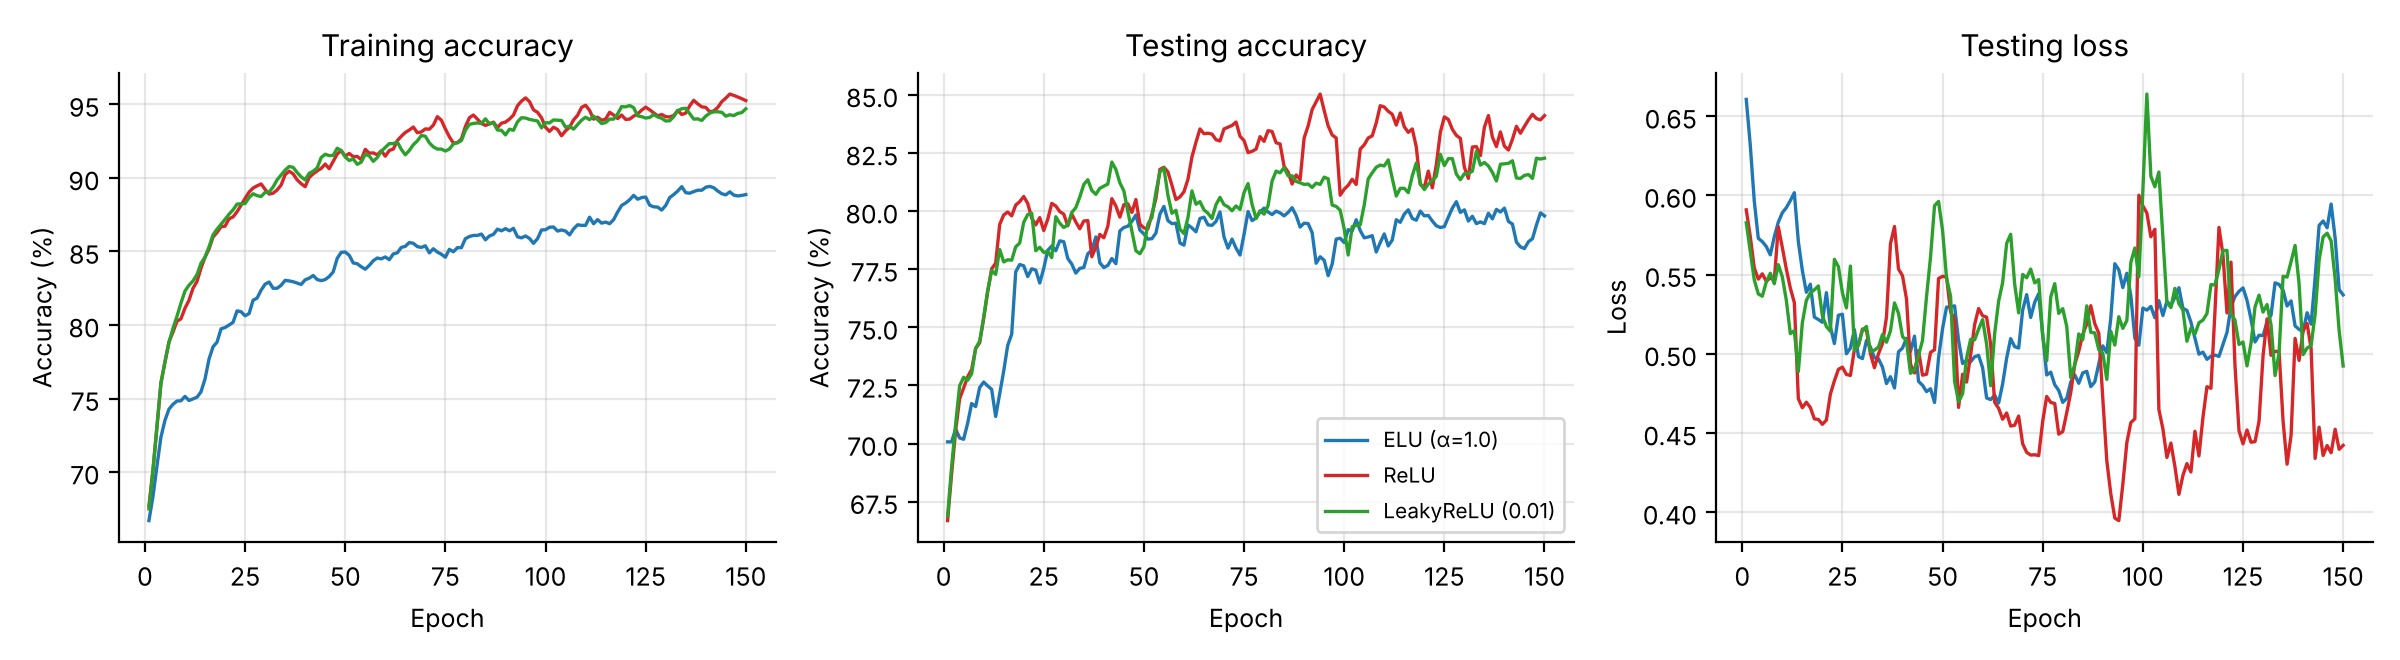
\includegraphics[width=\linewidth]{cmp_activation.png}
\caption{Activation functions: ELU ($\alpha=1$), ReLU and LeakyReLU.}
\label{fig:act}
\end{figure}

\begin{figure}[H]
\centering
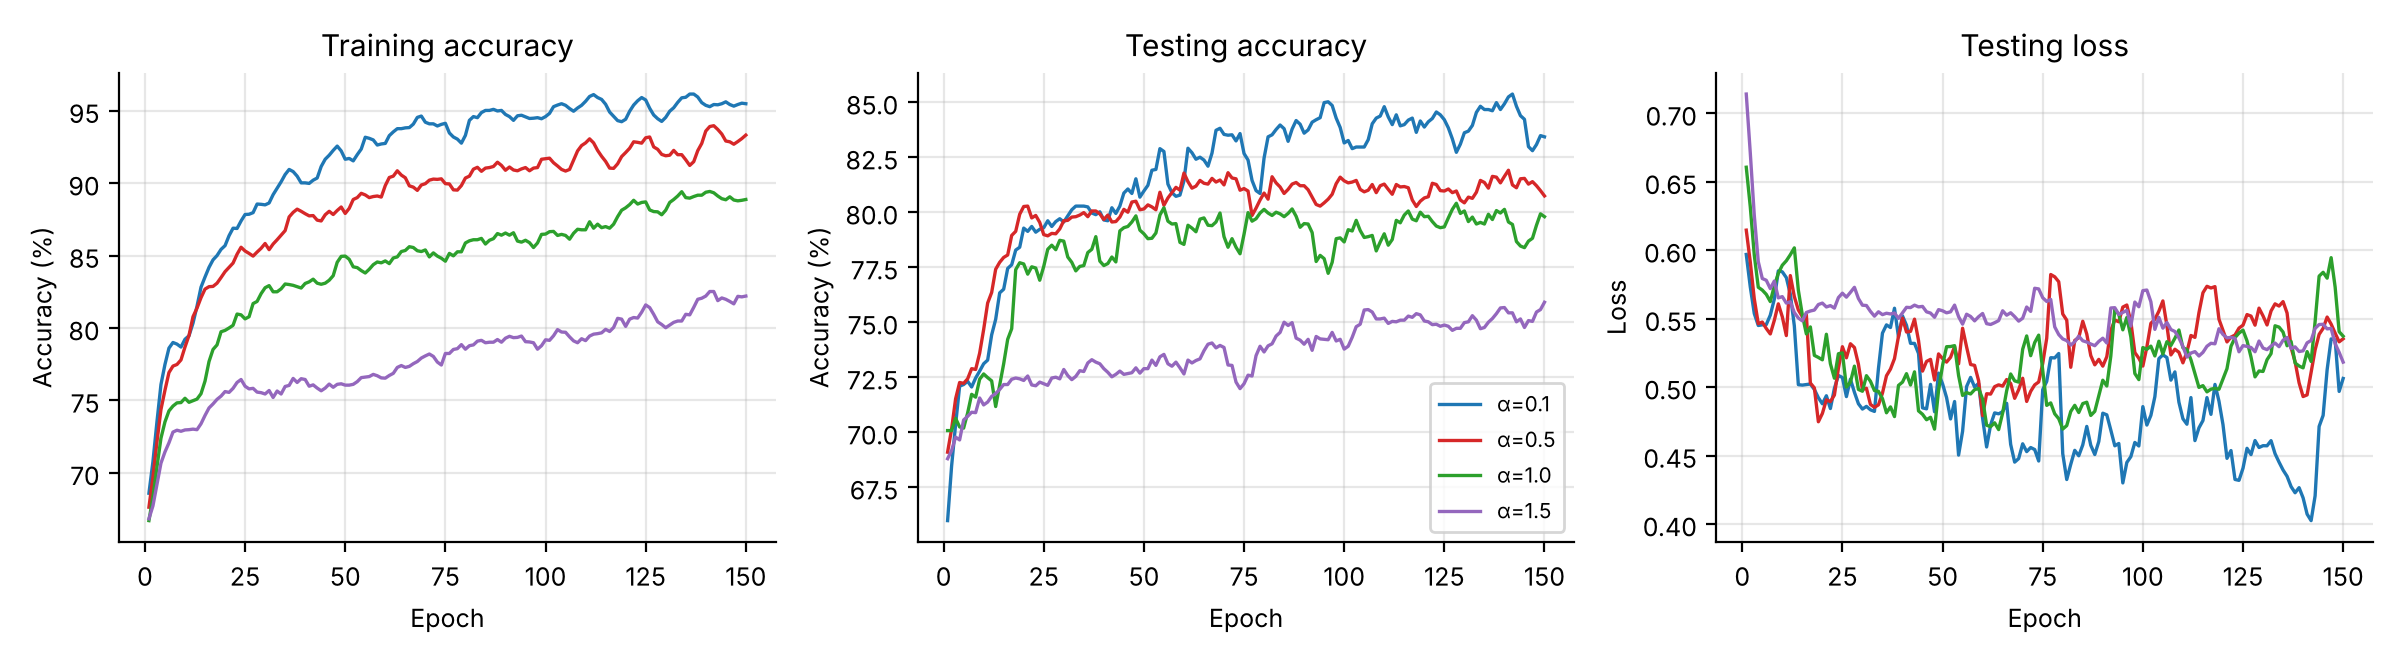
\includegraphics[width=\linewidth]{cmp_alpha.png}
\caption{ELU with $\alpha\in\{0.1,0.5,1.0,1.5\}$. Smaller $\alpha$ gives monotonically higher training and testing accuracy.}
\label{fig:alpha}
\end{figure}

\begin{figure}[H]
\centering
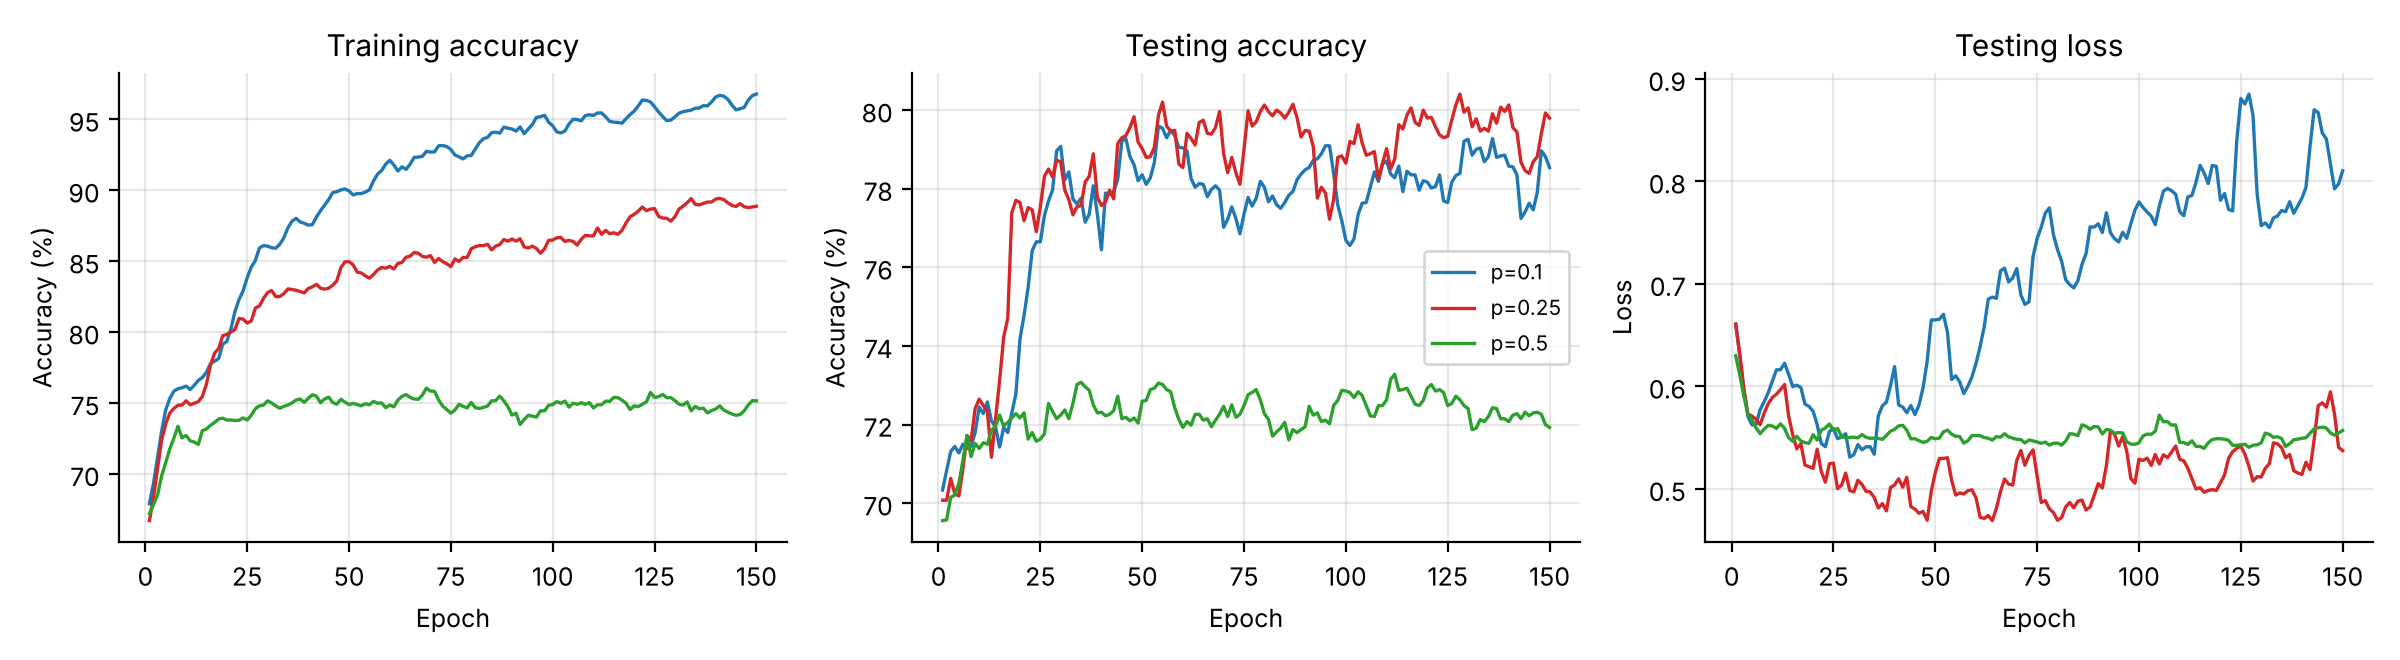
\includegraphics[width=\linewidth]{cmp_dropout.png}
\caption{Dropout rate. With $p=0.5$ the model underfits; with $p=0.1$ the testing loss rises again after about 35 epochs, which indicates overfitting.}
\label{fig:dropout}
\end{figure}

\begin{figure}[H]
\centering
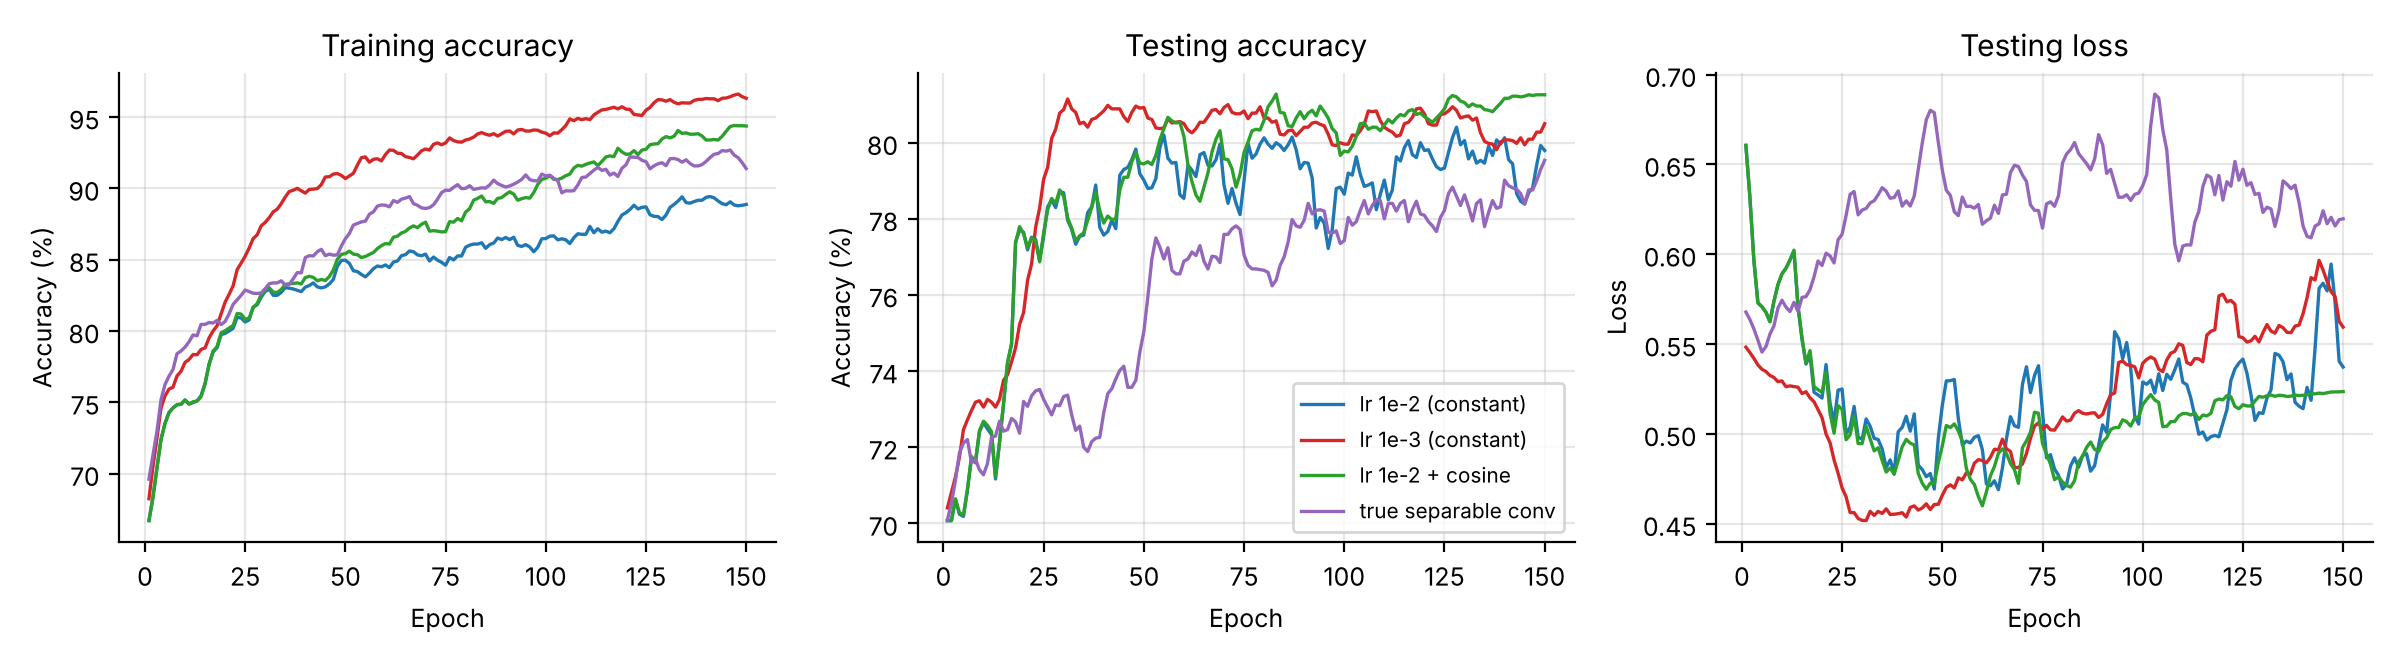
\includegraphics[width=\linewidth]{cmp_lr_sep.png}
\caption{Learning rate and schedule, and the true depthwise-separable convolution (lr $10^{-2}$, constant).}
\label{fig:lrsep}
\end{figure}

\subsection{Round 2: improving the best settings (300 epochs)}

Round~1 showed that the activation function matters most: ReLU and ELU with a small $\alpha$ were clearly the best. The baseline was also still improving at epoch 150. Round~2 therefore started from ELU with $\alpha=0.1$ or ReLU, trained for 300 epochs, and added the following techniques (all implemented in \texttt{main.py} as command-line options):
\begin{itemize}
  \item \textbf{Cosine annealing}: the learning rate decays from $10^{-2}$ to 0 over training.
  \item \textbf{Data augmentation}, applied to the training batches only:
  \begin{itemize}
    \item a random circular time shift of up to $\pm25$ samples (0.1\,s);
    \item random amplitude scaling by up to $\pm10\%$; and
    \item Gaussian noise with a standard deviation of 5\% of the signal standard deviation.
  \end{itemize}
  \item \textbf{Other options}: label smoothing, AdamW, and a wider EEGNet ($F_1=32$, $F_2=64$, 66{,}466 parameters).
\end{itemize}
The script \texttt{tune.py} first runs ten candidate settings (Table~\ref{tab:round2}). It then retrains the three best settings with seeds 1--3 to check that their accuracy is not due to a lucky initialisation (Figure~\ref{fig:seeds}).

\begin{table}[H]
\centering
\caption{Round 2 results for EEGNet (300 epochs, seed 0). Unless stated otherwise, lr is $10^{-2}$ and weight decay is $10^{-3}$. ``Aug.'' denotes the time shift, amplitude scaling and noise augmentation.}
\label{tab:round2}
\small
\resizebox{\linewidth}{!}{%
\begin{tabular}{lcccc}
\toprule
Setting & Highest test (\%) & Epoch & Mean last 10 (\%) & Final train (\%) \\
\midrule
ELU $\alpha$=0.1 + cosine + aug. & \textbf{88.06} & 234 & \textbf{86.99} & 97.04 \\
ELU $\alpha$=0.1, lr $10^{-3}$, wd $10^{-4}$ & 87.78 & 270 & 86.79 & 99.07 \\
ReLU, lr $10^{-3}$, wd $10^{-4}$ & 87.69 & 224 & 86.28 & 99.07 \\
ReLU + cosine + aug. & 87.59 & 179 & 86.77 & 97.50 \\
ELU $\alpha$=0.1 + cosine + aug. + label smoothing 0.1 & 86.85 & 273 & 85.64 & 96.39 \\
ReLU + cosine & 86.85 & 224 & 86.57 & 99.91 \\
ELU $\alpha$=0.1 + cosine & 86.76 & 222 & 86.42 & 99.63 \\
ReLU + AdamW (wd 0.01) + cosine + aug. & 86.76 & 273 & 86.49 & 98.24 \\
ReLU, wide EEGNet ($F_1$=32, $F_2$=64) + cosine + aug. & 86.67 & 264 & 85.56 & 98.06 \\
LeakyReLU + cosine & 85.00 & 277 & 84.47 & 99.35 \\
\bottomrule
\end{tabular}}
\end{table}

\begin{figure}[H]
\centering
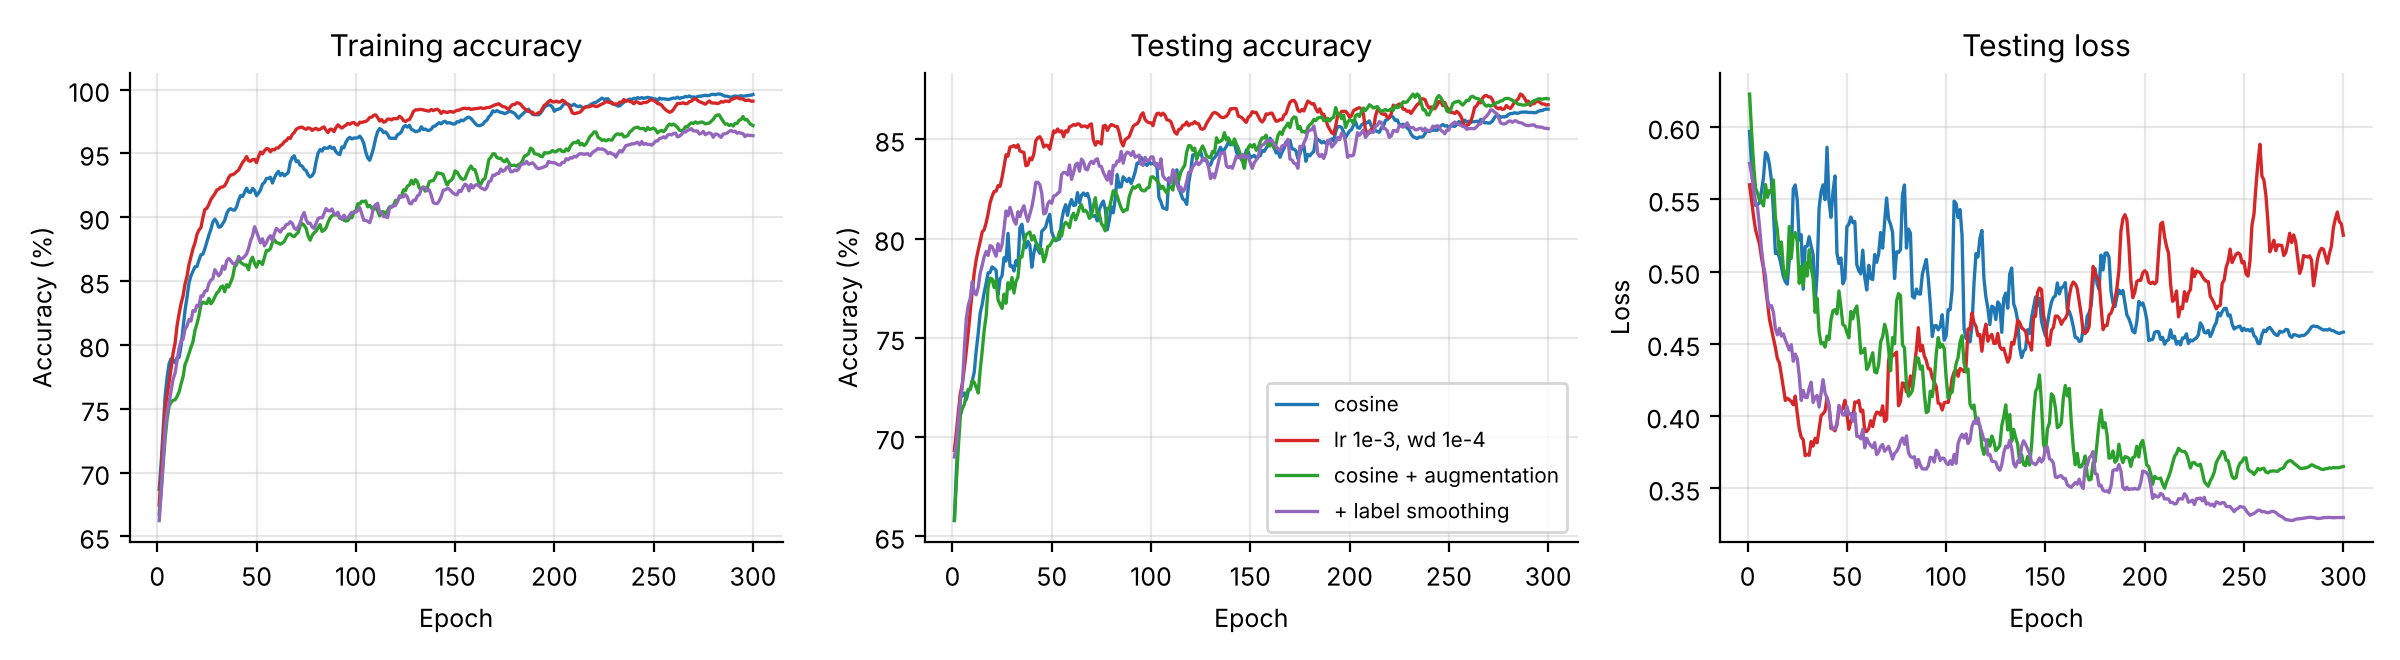
\includegraphics[width=\linewidth]{cmp_tuning.png}
\caption{Round 2 runs with ELU ($\alpha=0.1$) and 300 epochs. Augmentation keeps the testing loss lowest and the testing accuracy highest at the end of training.}
\label{fig:tuning}
\end{figure}

\begin{figure}[H]
\centering
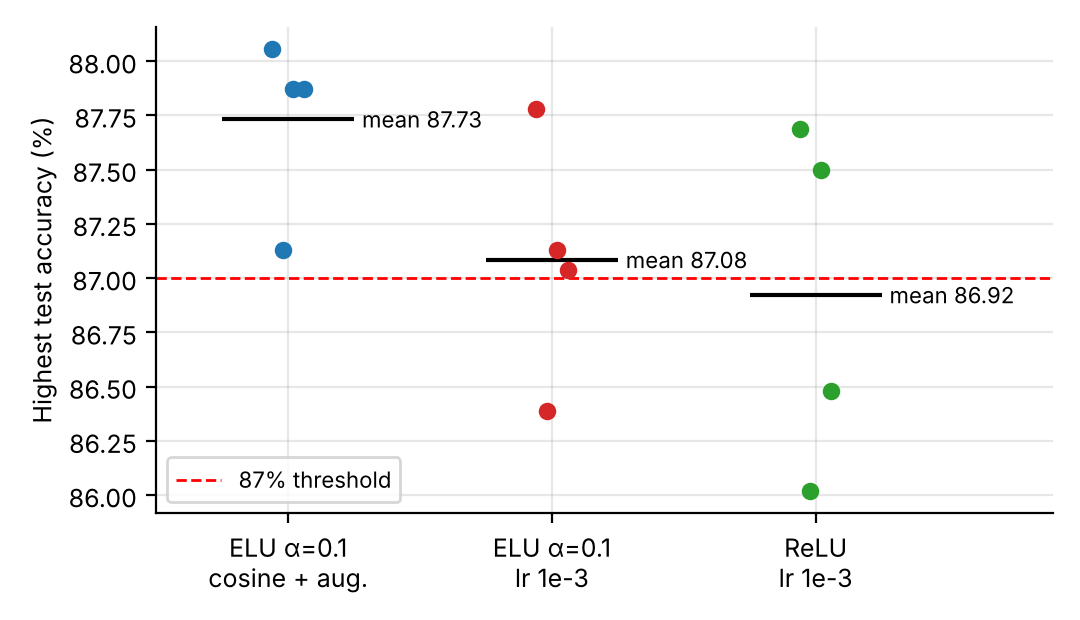
\includegraphics[width=0.62\linewidth]{seeds.png}
\caption{Highest testing accuracy of the three best round-2 settings over four seeds (0--3); the black bars are the means. All four seeds of the best setting are above 87\%.}
\label{fig:seeds}
\end{figure}

\subsection{Highest testing accuracy}

The highest testing accuracy is \textbf{88.06\%}. It was reached at epoch 234 by EEGNet with ELU ($\alpha=0.1$), dropout 0.25, Adam (lr $10^{-2}$, weight decay $10^{-3}$) with cosine annealing over 300 epochs, and data augmentation. The command was:
\begin{lstlisting}
python main.py -activation elu -alpha 0.1 -num_epochs 300 -cosine \
               -aug_shift 25 -aug_scale 0.1 -aug_noise 0.05 -seed 0
\end{lstlisting}
Figure~\ref{fig:screenshot} shows the saved best checkpoint reloaded in Colab and evaluated on the testing set; it reproduces 88.06\%.

\begin{figure}[H]
\centering
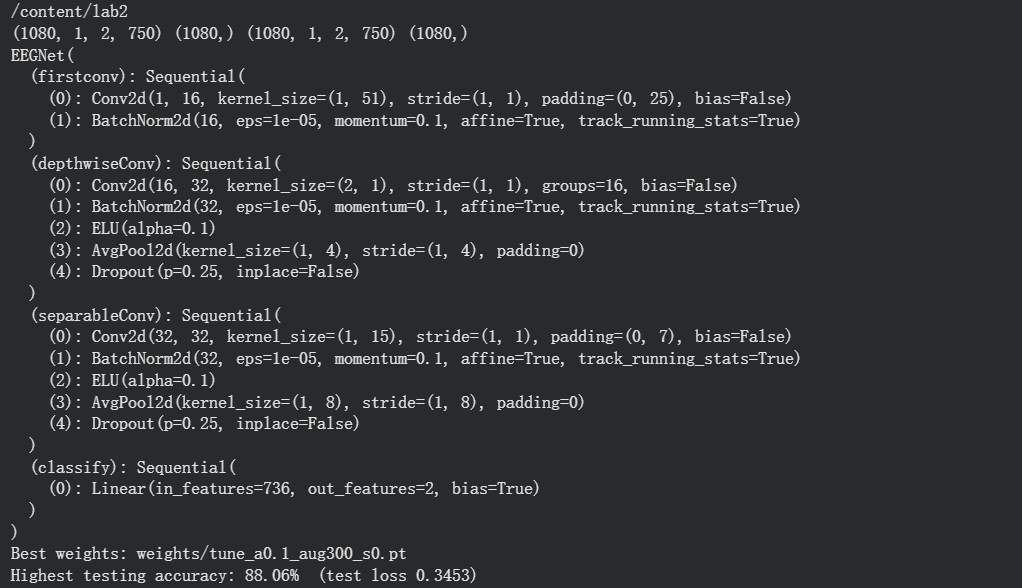
\includegraphics[width=0.85\linewidth]{best_test_screenshot.png}
\caption{Screenshot: the best checkpoint (\texttt{weights/tune\_a0.1\_aug300\_s0.pt}) reloaded and evaluated on the 1{,}080 testing trials.}
\label{fig:screenshot}
\end{figure}

\subsection{Training and testing loss and accuracy curves}

\begin{figure}[H]
\centering
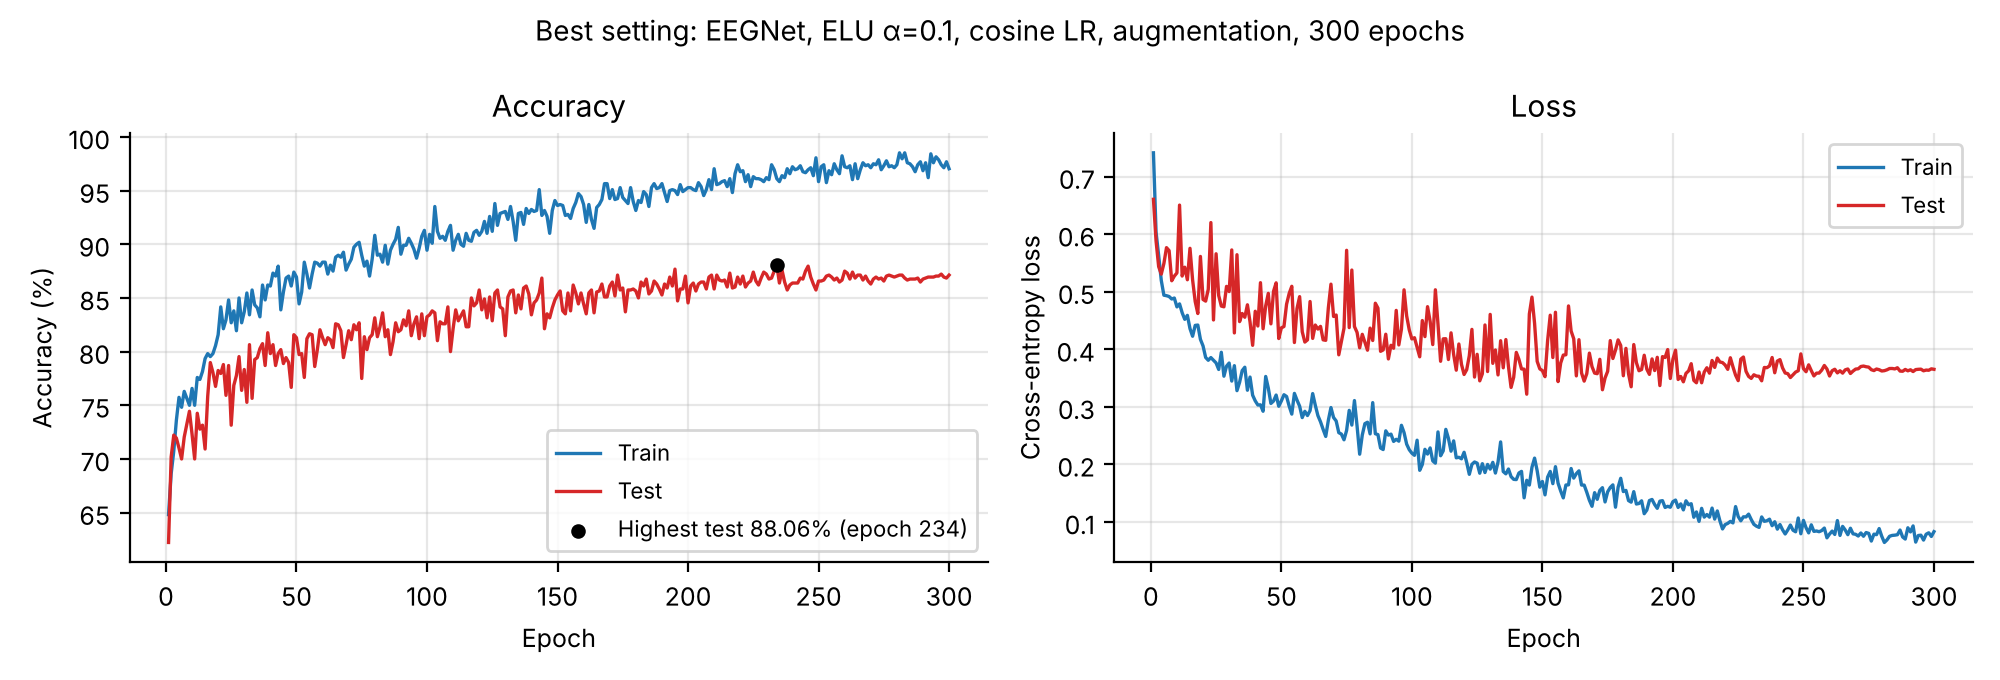
\includegraphics[width=\linewidth]{best_curves.png}
\caption{Training and testing accuracy and loss of the best model. The black dot marks the highest testing accuracy.}
\label{fig:best}
\end{figure}

\begin{figure}[H]
\centering
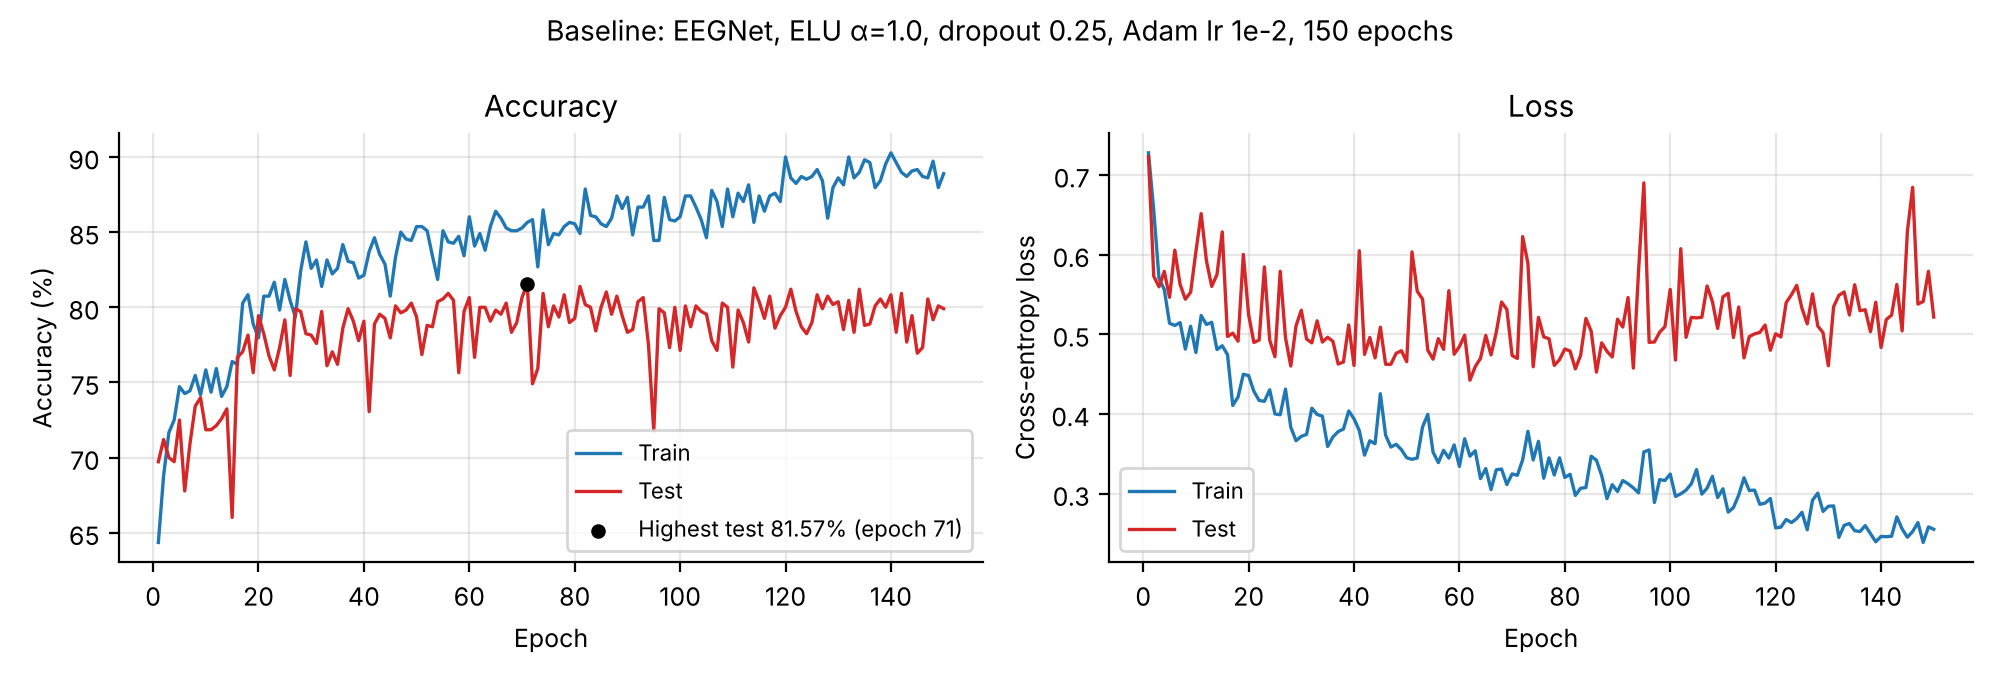
\includegraphics[width=\linewidth]{baseline_curves.png}
\caption{Training and testing accuracy and loss of the baseline EEGNet from the specification.}
\label{fig:baseline}
\end{figure}

%==========================================================================
\section{Discussion}

\subsection{Findings}

\paragraph{The activation function and ELU $\alpha$ matter most.}
In round 1, accuracy increased steadily as $\alpha$ decreased. Comparing $\alpha=1.5$ with $\alpha=0.1$:
\begin{itemize}
  \item the highest test accuracy rose from 76.67\% to 86.48\%;
  \item the mean test accuracy of the last 10 epochs rose from 75.24\% to 83.94\%; and
  \item the final training accuracy rose from 82.41\% to 95.56\%.
\end{itemize}
ReLU, which corresponds to the limit $\alpha\to0$, behaved almost the same as $\alpha=0.1$ (86.11\%). The training curves (Figure~\ref{fig:alpha}) show that a large $\alpha$ mainly slows down \emph{fitting}: it is an optimisation effect, not overfitting. Every activation follows a BatchNorm layer, so roughly half of its inputs are negative. With a large $\alpha$, these inputs produce outputs down to $-\alpha$ instead of approximately 0. The following average-pooling layer therefore mixes large negative and positive values, which blurs the features passed to the next block. In addition, under weight decay $10^{-3}$ with lr $10^{-2}$, the network fits the data less easily. A small $\alpha$ keeps the useful property of ELU (a non-zero gradient for $x<0$, so units never ``die'') while producing sparser, ReLU-like features. LeakyReLU (slope 0.01) was slightly worse than ReLU in both rounds.

\paragraph{Dropout controls the bias--variance trade-off.}
With $p=0.5$ the model underfits: it reaches only 75.09\% training accuracy and 75.00\% at best on the test set. With $p=0.1$ it fits the training set better (96.76\%), but the testing loss climbs from its minimum of 0.51 at epoch 34 to about 0.83 at the end, which is a clear sign of overfitting. The default $p=0.25$ lies between these two extremes.

\paragraph{Learning rate and schedule.}
With lr $10^{-3}$, the model fitted fastest. It peaked at epoch 31 and then slowly overfitted. Cosine annealing reduces the update noise at the end of training. It raised the mean of the last 10 epochs from 79.04\% to 81.24\% and flattened the testing curve, which makes the final model more reliable. With 300 epochs, both lr $10^{-3}$ (with a smaller weight decay) and lr $10^{-2}$ with cosine annealing exceeded 86.7\%.

\paragraph{Data augmentation reduces overfitting.}
Without augmentation, the 300-epoch runs reached 99.6--99.9\% training accuracy, and their testing loss rose again towards the end (Figure~\ref{fig:tuning}). With time shift, scaling and noise, training accuracy stayed at about 97\%, and the final testing loss decreased from 0.459 to 0.365. Both the highest accuracy (88.06\% vs.\ 86.76\%) and the mean of the last 10 epochs (86.99\% vs.\ 86.42\%) improved. A random time shift makes sense for motor imagery, because the onset of the imagined movement is not perfectly aligned across trials.

\paragraph{Things that did not help.}
\begin{itemize}
  \item \textbf{A wider EEGNet} ($3.7\times$ the parameters) did not improve accuracy (86.67\%). The 1{,}080 training trials, not the model capacity, are the limiting factor.
  \item \textbf{Label smoothing} lowered the peak to 86.85\%.
  \item \textbf{AdamW} with a stronger weight decay gave no clear gain.
\end{itemize}

\paragraph{The result is robust to the seed, but the ``highest'' metric is optimistic.}
Over seeds 0--3, the best setting reached 88.06, 87.13, 87.87 and 87.87\% (mean 87.73\%), so every seed passed 87\%. The other two candidates averaged 87.08\% and 86.92\%. Training is also not bit-exact on a GPU. Repeating the baseline gave 81.57\% and 81.94\%, and a re-run of the best setting gave 86.67\%. The highest testing accuracy is selected \emph{using the test set}, as this lab requires, so it is an optimistic estimate. The mean of the last 10 epochs (86.99\% for the best setting) is a fairer estimate of performance on unseen data; a separate validation split would be needed for unbiased model selection.

\subsection{How the model is implemented}

\paragraph{Data.} \texttt{dataloader.read\_bci\_data()} performs the following steps:
\begin{itemize}
  \item concatenates the two subjects;
  \item maps the labels $\{1,2\}\to\{0,1\}$;
  \item reshapes each trial from $[750,2]$ to $[1,2,750]$, i.e.\ one ``image'' with 2 rows (electrodes) and 750 columns (time); and
  \item replaces NaN values by the mean.
\end{itemize}
The path of the data folder is now resolved relative to the source file, so the code can be run from any directory. A small \texttt{Dataset} class returns float32 signals and int64 labels to a \texttt{DataLoader}; the training set is shuffled.

\paragraph{Model.} \texttt{models/EEGNet.py} builds the four blocks in Table~\ref{tab:arch} with \texttt{nn.Sequential}:
\begin{itemize}
  \item The temporal convolution uses a $(1,51)$ kernel with padding 25, so the time length stays at 750.
  \item The depthwise convolution uses a $(2,1)$ kernel that spans both electrodes, with \texttt{groups=16}. Each of the 16 temporal maps therefore gets $D=2$ spatial filters (16$\to$32 maps), and the electrode axis collapses to 1.
  \item The two average-pooling layers reduce the time axis $750\to187\to23$, which gives $32\times23=736$ features for \texttt{nn.Linear(736, 2)}.
  \item The convolutions have no bias, because each is followed by a BatchNorm layer, which provides its own shift.
  \item The activation is created by \texttt{get\_activation(name, alpha)}, so the activation function, $\alpha$, dropout rate, $F_1$, $D$, $F_2$ and the true-separable option are all command-line arguments.
\end{itemize}
The forward pass returns raw logits, because \texttt{CrossEntropyLoss} applies log-softmax internally.
\begin{lstlisting}
self.firstconv = nn.Sequential(
    nn.Conv2d(1, 16, kernel_size=(1, 51), padding=(0, 25), bias=False),
    nn.BatchNorm2d(16))
self.depthwiseConv = nn.Sequential(
    nn.Conv2d(16, 32, kernel_size=(2, 1), groups=16, bias=False),
    nn.BatchNorm2d(32), get_activation(activation, alpha),
    nn.AvgPool2d(kernel_size=(1, 4)), nn.Dropout(p=dropout))
self.separableConv = nn.Sequential(
    nn.Conv2d(32, 32, kernel_size=(1, 15), padding=(0, 7), bias=False),
    nn.BatchNorm2d(32), get_activation(activation, alpha),
    nn.AvgPool2d(kernel_size=(1, 8)), nn.Dropout(p=dropout))
self.classify = nn.Sequential(nn.Linear(736, 2))

def forward(self, x):                    # [B, 1, 2, 750]
    x = self.firstconv(x)                # [B, 16, 2, 750]
    x = self.depthwiseConv(x)            # [B, 32, 1, 187]
    x = self.separableConv(x)            # [B, 32, 1, 23]
    return self.classify(x.flatten(1))   # [B, 2] logits
\end{lstlisting}

\paragraph{Training and evaluation.}
\begin{itemize}
  \item \textbf{Training step}: each epoch runs \texttt{model.train()} and, for every mini-batch, augments the batch (if enabled) and then performs zero\_grad $\to$ forward $\to$ loss $\to$ backward $\to$ optimizer step. The loss multiplied by the batch size and the number of correct predictions are accumulated.
  \item \textbf{Evaluation}: the testing set is evaluated under \texttt{model.eval()} and \texttt{torch.no\_grad()}, so dropout is disabled and BatchNorm uses its running statistics.
  \item \textbf{Outputs}: the training and testing loss and accuracy of each epoch are saved to JSON and plotted with matplotlib. \texttt{run\_experiments.py} and \texttt{tune.py} reproduce every run in this report.
\end{itemize}

\subsection{The ELU function}

The exponential linear unit~\cite{elu} is
\begin{equation}
\mathrm{ELU}(x)=\begin{cases} x, & x>0,\\ \alpha\,(e^{x}-1), & x\le 0,\end{cases}
\qquad
\frac{d\,\mathrm{ELU}}{dx}=\begin{cases} 1, & x>0,\\ \alpha e^{x}=\mathrm{ELU}(x)+\alpha, & x\le0.\end{cases}
\end{equation}
Compared with ReLU, ELU has three advantages:
\begin{enumerate}
  \item Negative inputs still produce a non-zero output and gradient, so units cannot ``die''.
  \item The negative outputs push the mean activation towards zero. This reduces the bias shift between layers and speeds up learning.
  \item Unlike LeakyReLU, the negative branch saturates smoothly to $-\alpha$. Large negative inputs, such as noise, therefore give a bounded and almost constant output, which is a noise-robust ``off'' state.
\end{enumerate}
When $\alpha=1$, the function is also differentiable at 0. The parameter $\alpha$ sets the saturation level (Figure~\ref{fig:elu}). As $\alpha\to0$, ELU approaches ReLU, and as $\alpha$ grows, the negative region becomes deeper. In our experiments a small $\alpha$ (0.1) was clearly best. The price of ELU is one exponential per element, which makes it slightly slower than ReLU.

\begin{figure}[H]
\centering
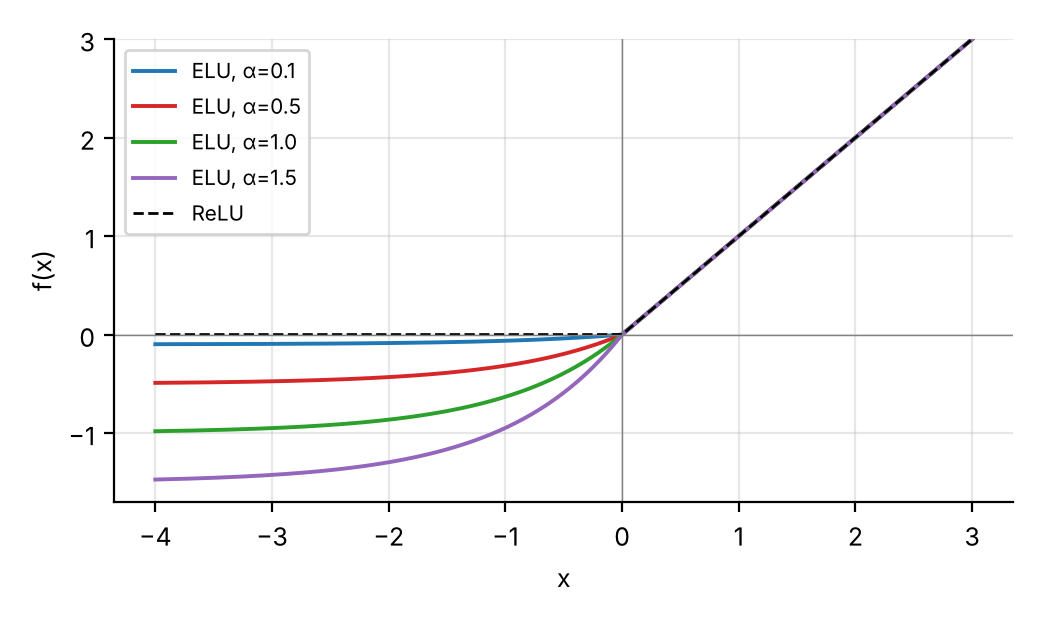
\includegraphics[width=0.55\linewidth]{elu.png}
\caption{ELU with different $\alpha$ compared with ReLU.}
\label{fig:elu}
\end{figure}

\subsection{Depthwise and separable convolution}

\paragraph{Standard convolution.} A $k_h\times k_w$ convolution from $C_{in}$ to $C_{out}$ channels has $C_{in}C_{out}k_hk_w$ weights. Every output channel sees every input channel, so a single layer performs both spatial (or temporal) filtering and channel mixing.

\paragraph{Depthwise convolution.} Each input channel is convolved only with its own filter(s); in PyTorch this is \texttt{groups} $=C_{in}$. With a depth multiplier $D$, each input channel produces $D$ output channels, so the layer has only $C_{in}Dk_hk_w$ weights and no information is exchanged between channels. In EEGNet the depthwise convolution has a $(2,1)$ kernel, i.e.\ (number of electrodes, 1). For each of the 16 band-pass-filtered maps it learns $D=2$ \emph{spatial filters}, which are weighted combinations of the electrodes; this is exactly the role of common spatial patterns (CSP) in classical BCI. Because each spatial filter is tied to one frequency band, the model stays interpretable. It also uses only 64 weights instead of the 1{,}024 that a full convolution would need.

\paragraph{Depthwise-separable convolution.} A standard convolution is factorised into two steps:
\begin{itemize}
  \item a depthwise convolution, which filters each channel along time; followed by
  \item a pointwise $1\times1$ convolution, which mixes the channels.
\end{itemize}
The number of weights drops from $C_{in}C_{out}k$ to $C_{in}k+C_{in}C_{out}$. In the original EEGNet, the third block is such a separable convolution: a depthwise convolution summarises each feature map over about 0.5\,s, and the $1\times1$ convolution learns how to combine the maps. The benefits are fewer parameters and multiply--adds, plus a built-in regularisation that suits small EEG datasets. The cost is lower expressive power, because the temporal filter of each map cannot depend on the other maps.

The model in this lab's specification uses a single full convolution, \texttt{Conv2d(32,32,(1,15))}, in the \texttt{separableConv} block. I therefore also implemented a true separable version (\texttt{-true\_separable}: a depthwise $(1,15)$ convolution with \texttt{groups=32}, followed by a $1\times1$ convolution). It has $10\times$ fewer weights in that layer (Table~\ref{tab:params}) and 4{,}018 parameters in total instead of 17{,}874. Under the default settings it reached 79.91\% versus 81.57\%. It reached a slightly higher final training accuracy (90.93\% vs.\ 88.89\%) but a higher testing loss (minimum 0.535 vs.\ 0.442), so it generalised slightly worse. On this 2-channel dataset the full convolution's extra mixing capacity helps a little. Still, the separable version stays within about 2\% while using 23\% of the parameters, which shows how efficient the factorisation is.

\begin{table}[H]
\centering
\caption{Weights of the convolution choices discussed (bias-free).}
\label{tab:params}
\small
\begin{tabular}{llr}
\toprule
Layer & Convolution type & Weights \\
\midrule
Spatial conv $16\to32$, $(2,1)$ & full convolution & 1{,}024 \\
Spatial conv $16\to32$, $(2,1)$ & depthwise, groups $=16$ (EEGNet) & 64 \\
Temporal conv $32\to32$, $(1,15)$ & full convolution (lab specification) & 15{,}360 \\
Temporal conv $32\to32$, $(1,15)$ & depthwise (480) + pointwise (1{,}024) & 1{,}504 \\
\bottomrule
\end{tabular}
\end{table}

%==========================================================================
\section{Bonus: DeepConvNet}

DeepConvNet~\cite{deepconvnet} is a deeper, general-purpose CNN. Its first block is a temporal convolution followed by a spatial convolution. Three more blocks follow, each consisting of convolution, BatchNorm, activation, max pooling and dropout, with 50, 100 and 200 filters. A dense layer produces the output. I implemented it from the table in the specification ($C=2$, $T=750$, $N=2$) without the max-norm constraint (Table~\ref{tab:deep}). It has 150{,}977 parameters and was trained with the same hyper-parameters as the EEGNet baseline (Adam lr $10^{-2}$, weight decay $10^{-3}$, batch size 64, 150 epochs), with dropout 0.5.

\begin{table}[H]
\centering
\caption{DeepConvNet as implemented.}
\label{tab:deep}
\small
\begin{tabular}{lll}
\toprule
Layer & Setting & Output shape \\
\midrule
Conv2d & $1\to25$, $(1,5)$ & $25\times2\times746$ \\
Conv2d + BN + act. & $25\to25$, $(2,1)$ & $25\times1\times746$ \\
MaxPool + Dropout & $(1,2)$, $p=0.5$ & $25\times1\times373$ \\
Conv2d + BN + act. + MaxPool + Dropout & $25\to50$, $(1,5)$ & $50\times1\times184$ \\
Conv2d + BN + act. + MaxPool + Dropout & $50\to100$, $(1,5)$ & $100\times1\times90$ \\
Conv2d + BN + act. + MaxPool + Dropout & $100\to200$, $(1,5)$ & $200\times1\times43$ \\
Flatten + Linear & $8600\to2$ & 2 \\
\bottomrule
\end{tabular}
\end{table}

\begin{table}[H]
\centering
\caption{DeepConvNet compared with EEGNet (150 epochs, same optimiser settings).}
\label{tab:deepres}
\small
\begin{tabular}{lccccr}
\toprule
Model & Highest test (\%) & Epoch & Mean last 10 (\%) & Final train (\%) & Params \\
\midrule
DeepConvNet, ELU & 80.37 & 131 & 77.60 & 86.85 & 150{,}977 \\
DeepConvNet, ReLU & \textbf{82.04} & 99 & \textbf{79.67} & 79.35 & 150{,}977 \\
DeepConvNet, LeakyReLU & 81.94 & 115 & 79.17 & 79.81 & 150{,}977 \\
\midrule
EEGNet, ELU $\alpha$=1 (baseline) & 81.57 & 71 & 79.04 & 88.89 & 17{,}874 \\
EEGNet, ReLU & 86.11 & 92 & 83.81 & 95.09 & 17{,}874 \\
EEGNet, best (round 2) & 88.06 & 234 & 86.99 & 97.04 & 17{,}874 \\
\bottomrule
\end{tabular}
\end{table}

\begin{figure}[H]
\centering
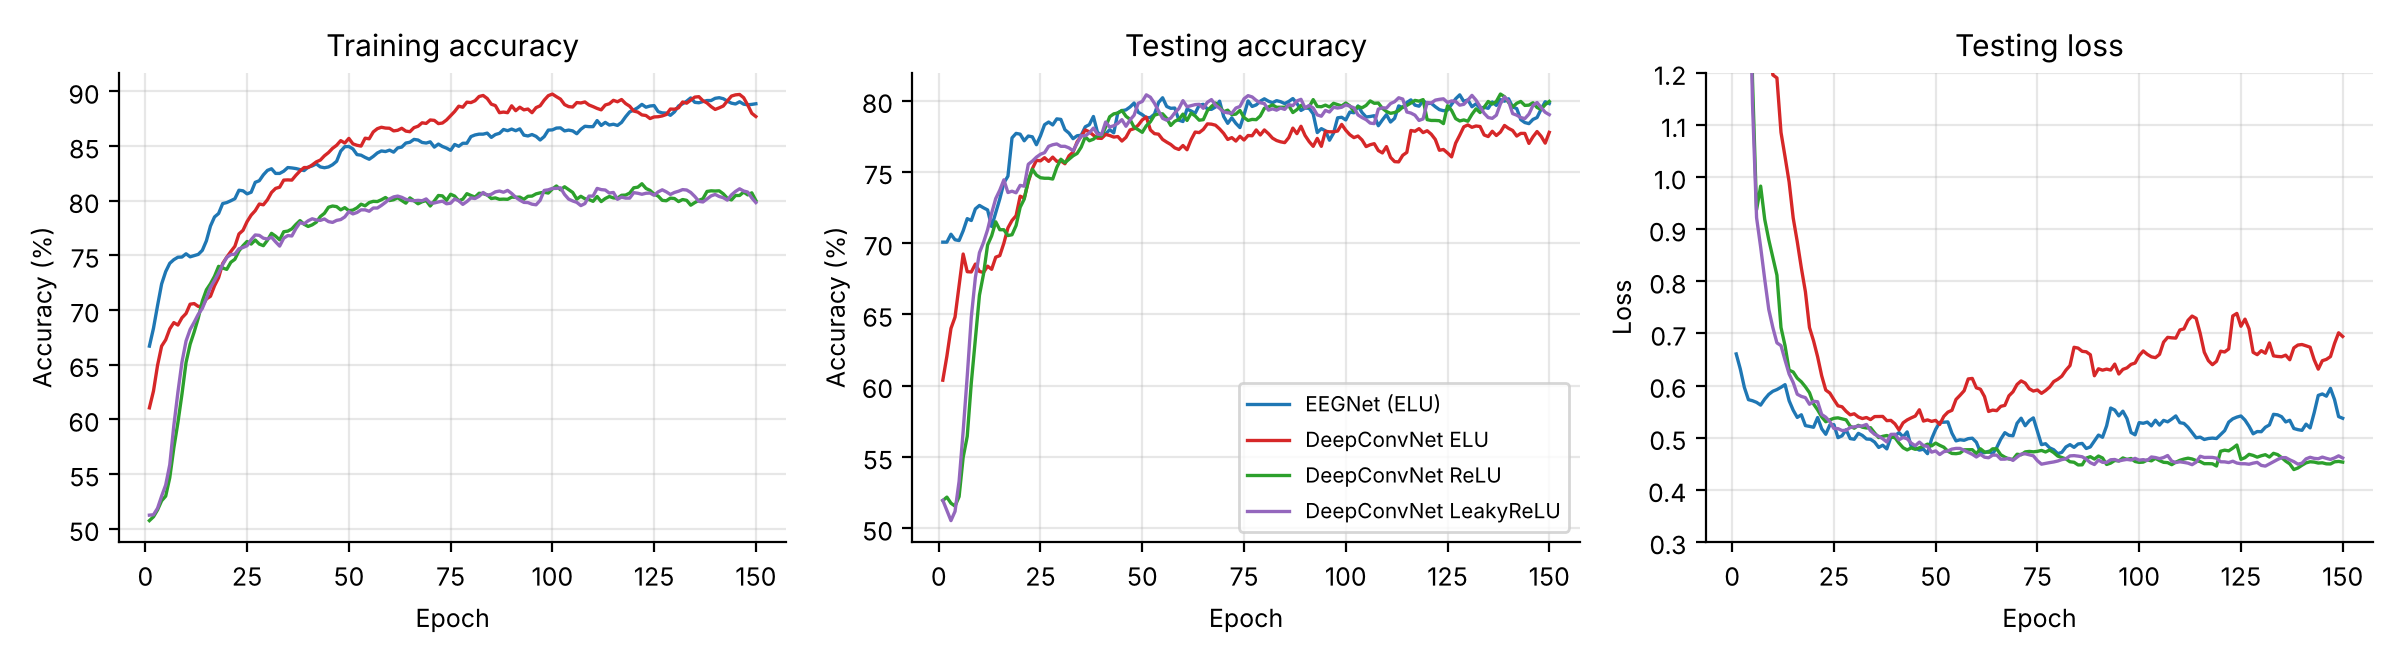
\includegraphics[width=\linewidth]{cmp_deepconvnet.png}
\caption{DeepConvNet with three activation functions compared with the EEGNet baseline (5-epoch moving average).}
\label{fig:deep}
\end{figure}

The best DeepConvNet reached 82.04\% with ReLU. That is comparable to the EEGNet baseline, but clearly below EEGNet with ReLU (86.11\%) and the best EEGNet (88.06\%), even though DeepConvNet has $8.4\times$ more parameters. Its training accuracy stayed at only 79--87\%. Three dropout layers with $p=0.5$, weight decay, and a large learning rate together make this deep network hard to fit with ReLU and LeakyReLU. With ELU it fits better (86.85\%), but its testing loss rises after about epoch 40, i.e.\ it starts to overfit (Figure~\ref{fig:deep}). On DeepConvNet the activation ranking is also different: ReLU and LeakyReLU beat ELU ($\alpha=1$). This agrees with the round-1 EEGNet result that a strongly negative ELU branch is not helpful here. Overall, EEGNet's compact, EEG-specific design reaches higher accuracy with far fewer parameters, which is the main argument of the EEGNet paper~\cite{eegnet}.

%==========================================================================
\begin{thebibliography}{9}
\bibitem{eegnet} V.~J.~Lawhern, A.~J.~Solon, N.~R.~Waytowich, S.~M.~Gordon, C.~P.~Hung, and B.~J.~Lance, ``EEGNet: A compact convolutional neural network for EEG-based brain--computer interfaces,'' \emph{Journal of Neural Engineering}, vol.~15, no.~5, 056013, 2018.
\bibitem{deepconvnet} R.~T.~Schirrmeister \emph{et al.}, ``Deep learning with convolutional neural networks for EEG decoding and visualization,'' \emph{Human Brain Mapping}, vol.~38, no.~11, pp.~5391--5420, 2017.
\bibitem{elu} D.-A.~Clevert, T.~Unterthiner, and S.~Hochreiter, ``Fast and accurate deep network learning by exponential linear units (ELUs),'' in \emph{ICLR}, 2016.
\bibitem{bci3b} BCI Competition III, data set IIIb, \url{http://www.bbci.de/competition/iii/desc_IIIb.pdf}.
\end{thebibliography}

\end{document}
